\begin{paracol}{2}
\begin{leftcolumn}
\noindent How does one start a project?

\begin{ally}
  With a bang, or with a whimper?
\end{ally}
Very funny.

In all seriousness, though. How? Does one come up with an idea and just\ldots{}what, go? Just start going and when you get to the end, stop? Can everything be, as NaNoWriMo would have it, pantsed? Run by the seat of your pants such that everything is done without planning, and thus nothing is unsurprising to the author?

Or does one plan meticulously? Does one craft an outline of such startling beauty that to finish the project itself feels almost a betrayal?

\begin{ally}
  Which are you guilty of?
\end{ally}
\end{leftcolumn}
\begin{rightcolumn*}
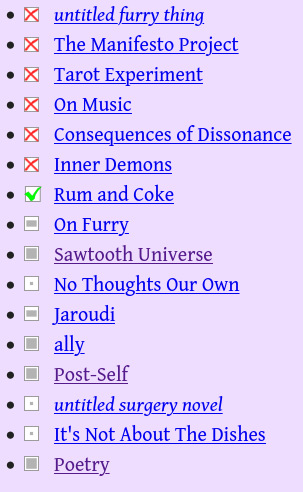
\includegraphics[width=2in]{assets/project-list.png}
\end{rightcolumn*}
\begin{leftcolumn}
Both, of course. I have my fair share of projects I planned so thoroughly that they fell through, just as I have my fair share of projects that I tried worked and worked and worked on and kept adding and adding and adding, and by the end they were so wandery as to be incomprehensible. They didn't hold together, and the story had gone so far off the rails that it was unfixable without a total rewrite.

\begin{ally}
  And which type was I?
\end{ally}
Don't preempt me. All of the projects that I've actually succeeded at have been somewhere in the middle. It's important to plan, as I've learned from all those countless unfinished projects, but there is also a fine balance of planning required, lest you plan your work out of existence.

\emph{Qoheleth}, the book that follows \emph{ally}, has, as a major theme, the difference between honing and forging. To hone is to take an idea and work it to an ever sharper point, whereas to forge is to take an idea, work until its good enough, and forge onwards. 

Neither is bad, of course. There is no value judgement in this distinction. Neither, also, is there any sense of permanence to the label. \emph{ally} was a project borne of forging: I was always trying to do something new with the typography, the wordchoice, the colors and textures of each of the sidequests, and so on. \emph{Restless Town} was a project borne of honing, though. My goal with those stories was to try and somehow come to the finest possible point of the lives involved and the tropes and identities that drive them. I wanted to take aspects of myself --- my gender, my mental health, my sexuality, my polyamory --- and hone each into a story worth reading.

But, as with outlining versus pantsing, one can go too far in either direction.

\begin{ally}
  And still, you will never not giggle when you write `pantsing'.
\end{ally}
Correct.

All that to say that, as Herbert would hvae it, beginnings are such delicate times. To start a project is to kill a portion of yourself, because, whether or not you succeed in finishing the project, whether or not you are trying to hone something to a cruel point or to forge into new territory, you will never start that project again. You will never again be the you who started that project.

\newpage

\begin{ally}
  And so why am I here?
\end{ally}
May I throw your words back at you?

\begin{ally}
  By all means.
\end{ally}
\emph{``Can an ally disinhabit a mind so easily?''}

\begin{ally}
  A question I remember you being decidedly uncomfortable with.
\end{ally}
Yes.

\begin{ally}
  But why am I here \textbf{now}? Why when we are talking about how this project was made?
\end{ally}
Do you not deserve to be here for such a conversation? I trust that you will have little to say of much of the mechanics, but much to say about the process of research.

\begin{ally}
  I do not doubt you. And yet you began this as a list of neat \LaTeX\ things you learned along the way. How often does one write a \LaTeX\ cookbook with one's imaginary friend?
\end{ally}
I don't know. Probably not often. There is precedent, though, for overused literary devices in technical writing. \texttt{Coy}\footnote{\href{https://metacpan.org/pod/Coy}{Coy module on CPAN}}, anyone? 

\begin{verse}
  Error messages\\
  strewn across my terminal.\\
  A vein starts to throb. 
   
  Their reproof adds the\\
  injury of insult to\\
  the shame of failure. 
   
  When a program dies\\
  what you need is a moment\\
  of serenity. 
\end{verse}

Or perhaps you enjoy foxes as I do:

\noindent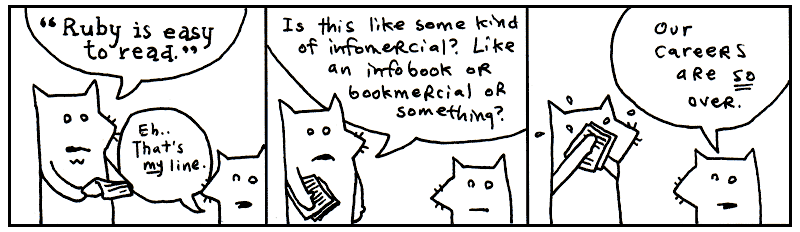
\includegraphics[width=4.2in]{assets/the.foxes-3.png}
\begin{center}
  \footnotesize
  From \href{https://poignant.guide}{\emph{Why's Poignant Guide to Ruby}} by \textbf{Why The Lucky Stiff}, licensed under a CreativeCommons Attribution-ShareAlike license.
\end{center}

There are all sorts of instances of folks writing technical things in a decidedly non-technical fashion.

\begin{ally}
  If you say so. What, then, are you going to talk about in this technical guide?
\end{ally}
Thanks for writing my segue for me.

\begin{labeling}{\textbf{The ally book}}
  \item[\textbf{ally.id}] How the interactive side of ally is built, including some fun examples.

  \emph{Page \pageref{site}}
  \item[\textbf{The ally book}] How the book itself was built.

  \emph{Page \pageref{book}}
  \item[\textbf{Gotchas}] Some problems I ran into along the way.

  \emph{Page \pageref{gotchas}}
\end{labeling}

\end{leftcolumn}
\end{paracol}
